\documentclass[conference]{IEEEtran}
\IEEEoverridecommandlockouts
% The preceding line is only needed to identify funding in the first footnote. If that is unneeded, please comment it out.
\usepackage{cite}
\usepackage{amsmath,amssymb,amsfonts}
\usepackage{algorithmic}
\usepackage{graphicx}
\usepackage{textcomp}
\usepackage{xcolor}
\usepackage{url}
\def\BibTeX{{\rm B\kern-.05em{\sc i\kern-.025em b}\kern-.08em
    T\kern-.1667em\lower.7ex\hbox{E}\kern-.125emX}}
\begin{document}

\title{Dengue outbreak prediction in Sri Lanka using machine learning techniques\\}

\author{\IEEEauthorblockN{Lakshitha Konara}
    \IEEEauthorblockA{\textit{Department of Computer Engineering} \\
        \textit{University of Peradeniya}\\
        Peradeniya, Sri lanka \\
        e18181@eng.pdn.ac.lk}
    \and
    \IEEEauthorblockN{Ravindu Mihiranga}
    \IEEEauthorblockA{\textit{Department of Computer Engineering} \\
        \textit{University of Peradeniya}\\
        Peradeniya, Sri lanka \\
        e18224@eng.pdn.ac.lk}
    \and
    \IEEEauthorblockN{Hirusha Uthsara}
    \IEEEauthorblockA{\textit{Department of Computer Engineering} \\
        \textit{University of Peradeniya}\\
        Peradeniya, Sri lanka \\
        e18368@eng.pdn.ac.lk}
    \and
    \IEEEauthorblockN{Dr. Namal Karunarathna}
    \IEEEauthorblockA{\textit{Department of Computer Engineering} \\
        \textit{University of Peradeniya}\\
        Peradeniya, Sri lanka \\
        namal@eng.pdn.ac.lk}
}

\maketitle

\begin{abstract}
    This paper focuses on the prediction of dengue fever outbreaks, which have become a significant
    public health concern in many tropical and subtropical regions worldwide. The study explores
    the complex and dynamic nature of the disease, considering various factors that influence its spread.
    By utilizing vector populations, urbanization, climate parameters and other relevant factors, 
    the research aims to develop effective strategies for early detection and prevention of dengue 
    outbreaks in Sri Lanka with the aid of machine learning techniques.

\end{abstract}


\section{Introduction}

Dengue fever has emerged as a significant public health concern in many tropical and
subtropical regions worldwide. It is estimated that about half of the world’s population
is at risk, with 100–400 million infections occurring annually[1].
In 2023, over six million dengue cases and over 6000 dengue-related deaths were reported
from 92 countries/territories. The highest burden of dengue was observed in the Americas,
where all four dengue virus serotypes circulated and caused outbreaks in several countries.
Brazil, Bangladesh, Mexico, Peru and Burkina Faso were among the countries with
the most cases. Dengue also occurred in Africa, Asia and Europe, where some
locally acquired cases were reported in Italy, France and Spain[2].
The disease is prevalent in tropical and sub-tropical climates, particularly in urban and
semi-urban areas. While many individuals infected with the dengue virus (DENV) remain
asymptomatic or experience only mild symptoms, the virus can occasionally lead to
evere illness and even death[1].

\begin{figure}[htbp]
    \centering
    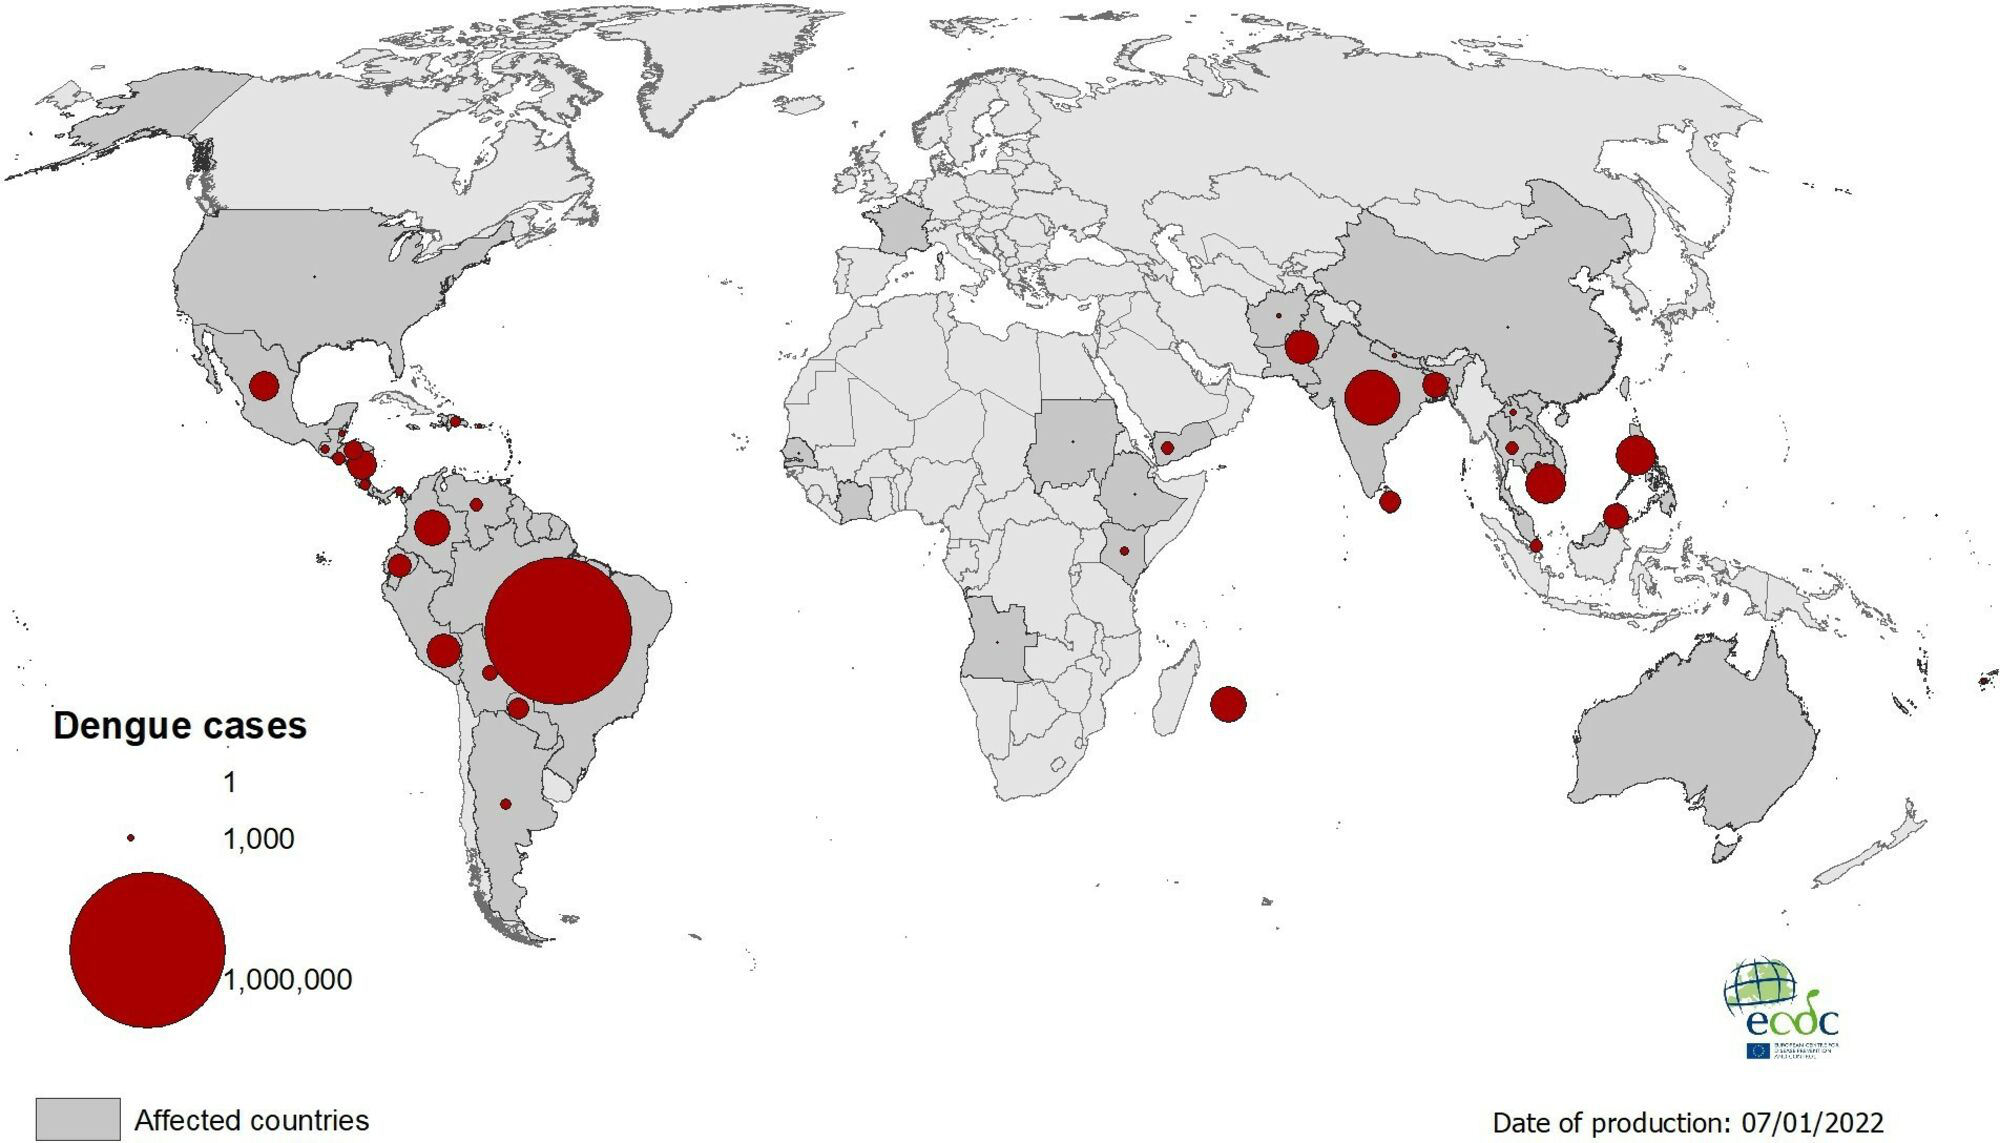
\includegraphics[width=0.5\textwidth]{fig1.png}
    \caption{Geographical distribution of dengue cases reported worldwide, 2021.}
\end{figure}

Dengue, a mosquito-borne viral disease caused by four distinct but closely
related serotypes of the dengue virus (DENV-1, DENV-2, DENV-3, and DENV-4), poses a
significant global health challenge. It is estimated that nearly 3.6 billion people
are at risk, with approximately 390 million infections annually, of which 96 million are
symptomatic. The disease spectrum ranges from asymptomatic dengue infection to severe
forms such as dengue hemorrhagic fever (DHF) and dengue shock syndrome (DSS), leading to
around 21,000 fatalities each year[3]. \\

Dengue is a complex and dynamic disease that is influenced by multiple
factors at different scales, from the molecular to the global.
Some of the factors that affect the spread of dengue include the
vector population, which determines the availability and distribution
of the mosquito vectors that transmit the dengue virus (DENV) to humans;
urbanization, which creates favorable conditions for vector breeding and
human exposure; climate change, which affects the ecology and behavior of
the mosquito vectors and the DENV; travel and globalization, which can
introduce new DENV strains or serotypes, or new mosquito vectors, to
previously unaffected areas; population density, which affects the contact
rate between humans and mosquitoes, and the herd immunity of the population;
immunity levels, which depend on the history and frequency of dengue
infections, and the cross-reactivity and duration of the antibodies;
and mutation and evolution of DENV, which can generate new variants with
different virulence, transmissibility, and antigenicity. \\

Dengue is a viral disease transmitted to humans through the bite of infected
mosquitoes, specifically a few species that act as vectors. A vector,
often an arthropod like mosquitoes, ticks, lice, flies, and fleas,
is an organism that carries and transmits a disease to its host. When a mosquito bites a
person infected with the dengue virus, it becomes a carrier of the virus and can infect
healthy individuals through subsequent bites. It’s important to note that dengue doesn’t
spread directly from person to person; mosquitoes are essential for its transmission.
Other diseases carried by vectors include Lyme disease by ticks and yellow fever, malaria,
and dengue fever by certain mosquitoes.[4]

Dengue is primarily spread by the Aedes aegypti mosquito, which serves as the main vector
for the virus. Other Aedes species, such as Aedes albopictus, Aedes polynesiensis,
and Aedes scutellaris, can also carry the virus but to a lesser extent. Aedes aegypti,
identifiable by white bands on its legs and a lyre-like pattern on its body,
thrives in tropical and subtropical regions, specifically between the latitudes
of 35°N and 35°S where winter temperatures stay above 10°C. They typically don’t
survive in altitudes above 1000 m due to colder temperatures. These mosquitoes are
closely associated with human habitats and usually spend their entire lives around their
hatching sites[4].

\begin{figure}[htbp]
    \centering
    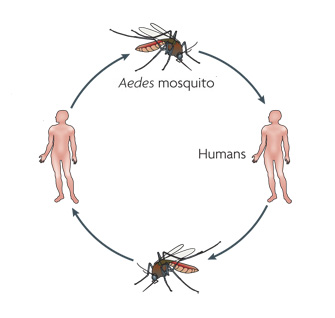
\includegraphics[width=0.5\textwidth]{fig2.png}
    \caption{Dengue transmission.}
\end{figure}

Dengue is transmitted to humans through the bite of an infected Aedes aegypti mosquito.
The mosquito becomes a dengue vector after feeding on a person with high levels of the virus
in their blood during a period known as viremia. The virus then spreads through the
mosquito’s body over 8-12 days, after which it can transmit the virus to other humans for
the rest of its life. Female mosquitoes, which require blood to produce eggs, inject their
saliva into the human host during feeding, thereby transmitting the virus. While the
majority of dengue transmissions occur through mosquito bites, rare instances of transmission
can occur through organ transplants, blood transfusions, or from an infected mother to her
fetus[4].

Dengue, a disease that can range from mild to severe, typically presents
symptoms 4-10 days post-infection, lasting 2-7 days. Common symptoms
include high fever, severe headache, eye pain, muscle and joint pains,
nausea, vomiting, swollen glands, and rash. A second infection
can increase the risk of severe dengue. After the fever subsides,
severe symptoms such as abdominal pain, persistent vomiting, rapid breathing,
bleeding gums or nose, fatigue, restlessness, blood in vomit or stool,
extreme thirst, pale and cold skin, and weakness may occur. Immediate
medical attention is advised for these severe symptoms. Post-recovery,
individuals may experience fatigue for several weeks[1]. \\

Dengue fever, a disease that can range from mild to severe, is primarily
managed at home with pain medication, with a focus on symptom control.
Acetaminophen (paracetamol) is commonly used for this purpose, while
non-steroidal anti-inflammatory drugs like ibuprofen and aspirin are
avoided due to their potential to increase bleeding risk. For individuals
who have contracted dengue at least once and reside in endemic areas,
the Dengvaxia vaccine is available. Severe cases often necessitate
hospitalization[1]. \\

Prevention and control of dengue are largely dependent on vector control
to avoid mosquito bites. Despite the lack of a specific treatment for
dengue and severe dengue, early detection and access to proper medical
care can significantly reduce fatality rates. Therefore, prevention
strategies and timely medical intervention are crucial in managing
this disease. \\

Sri Lanka, a lush tropical island in the Indian Ocean, home to 21 million
people, has been besieged by the relentless scourge of dengue fever since
the 1960s. Despite its seasonal nature, with epidemics primarily afflicting
regions experiencing annual rainfall exceeding 2,500 mm, the situation
escalated dramatically in 2017. Prior to 1988, occurrences of the more
severe dengue hemorrhagic fever were sporadic. However, from 1991 to 2008,
dengue epidemics became more pronounced, occurring every few years amidst
endemic transmission. The year 2009 marked a grim milestone with over 35,000
suspected cases and 346 deaths, highlighting the severity of the crisis.
Subsequent years saw a steady rise in cases, peaking in 2017 with a
staggering 186,101 suspected cases and 440 deaths, marking it as the
deadliest outbreak since dengue was classified as a notifiable disease in 1996. \\

The lack of a robust public health surveillance system compounded the
challenge, hindering efforts to track and monitor outbreaks effectively.
This deficiency, coupled with limited accessibility to medical facilities,
particularly in rural areas, exacerbated the crisis. High population density,
especially prevalent in the Eastern Province, further fueled the rapid
transmission of the disease, making containment efforts even more daunting.
Furthermore, the absence of regular updates on confirmed cases exacerbated
the difficulty in identifying trends and anticipating outbreaks.

The escalating threat of dengue fever in Sri Lanka is compounded by climatic
factors conducive to mosquito breeding, such as prolonged heatwaves.
The year 2020 witnessed a notable increase in cases, attributed in
large part to unusually hot weather conditions that persisted from
April to October. The soaring temperatures, reaching above 35°C (95°F)
almost daily, created ideal breeding grounds for mosquitoes. The influx of
people to beaches and water bodies during this period further exacerbated
the issue, leading to a surge in dengue fever cases across the country.
Urgent measures are needed to address this escalating public health crisis,
including the implementation of predictive tools to anticipate outbreaks and
the establishment of a comprehensive surveillance system to track and
monitor cases effectively.[5]

\begin{figure}[htbp]
    \centering
    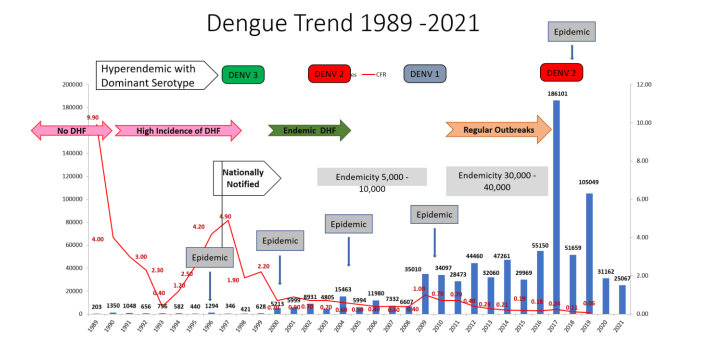
\includegraphics[width=0.5\textwidth]{fig3.png}
    \caption{The Reported Dengue Infected Count in Sri Lanka from 1989 to 2021.}
\end{figure}


\section{Related Work}

In examining various viral diseases prevalent in Sri Lanka, including Influenza,
HIV, SARS-CoV-2 and dengue viruses, it becomes evident that dengue poses a
particularly formidable challenge to public health in the region. Over the
past few decades, Sri Lanka has witnessed a significant number of recorded
cases of dengue fever, marking it as one of the most dangerous viruses in
the country. Despite the gravity of the situation posed by dengue, there is a
noticeable dearth of comprehensive data sets and research initiatives on other
viruses such as Influenza, HIV, and SARS-CoV-2 within Sri Lanka. Contrary to the
considerable attention garnered by dengue, these viruses have not been extensively
studied, revealing a significant research gap in understanding their epidemiology
and impact in the Sri Lankan context. \\

It is apparent that the current economic
conditions in Sri Lanka pose significant challenges to researchers, limiting their
motivation and resources to delve into comprehensive studies on viruses beyond dengue.
Moreover, the perennial occurrence of dengue fever in Sri Lanka underscores its
status as an unresolved critical public health issue. The cyclic nature of dengue
outbreaks underscores the urgent need for heightened research efforts and innovative
interventions to mitigate its impact on the Sri Lankan population. Thus, while dengue
remains a recurrent and pressing concern, the lack of attention towards other viral
diseases underscores the necessity for concerted research efforts and resource
allocation to address the broader spectrum of infectious diseases in Sri Lanka. \\

Machine learning (ML) stands as a transformative force in addressing the complexities
of dengue management and prediction. By harnessing algorithms and diverse datasets encompassing
clinical records, climatic trends, and socio-political factors, ML has become
indispensable in forecasting outbreaks and optimizing intervention strategies. Studies
conducted in Sri Lanka showcase the efficacy of ML in predicting dengue incidence,
from forecasting plasma leakage in suspected dengue patients to estimating outbreak
trends based on weather and geographical factors and developing a mathematical model
for estimating the number of dengue cases[6,7,8]. ML not only offers a promising
avenue for replacing costly and limited traditional methods but also provides timely
and accurate insights crucial for tackling the significant public health and economic burden
posed by dengue in regions like Sri Lanka. \\

Here are several ways in which ML can be useful,
One crucial area is epidemiological prediction, where ML models utilize historical data
to classify future dengue incidence as either high or low. Techniques like Fuzzy
Association Rule Mining have been instrumental in extracting intricate relationships
from diverse datasets, aiding in forecasting outbreaks in regions like Peru[9].
Another significant avenue is the use of ML to predict outbreaks based on climate variables.
Studies employing techniques such as Support Vector Machines have demonstrated the
efficacy of analyzing factors like temperature, humidity, and rainfall in forecasting
dengue outbreaks. These models provide timely information for health authorities to
implement preventive measures[10]. Temporal dynamics analysis is another essential
approach, involving a multi-stage ML approach to dissect the temporal relationship between
temperature fluctuations and dengue occurrences. By integrating auto-encoding, data representation,
and temporal clustering, these models offer accurate predictions of outbreak trends over time[11].
Comparative performance evaluation between ML algorithms and traditional regression
models is pivotal in understanding their effectiveness in dengue prediction. ML
models have showcased superior performance, especially in scenarios where surveillance
data are readily available, such as weekly case count predictions[12]. Furthermore, ML
enables dynamic ensemble learning, where ML can dynamically identify local patterns in weather
and population susceptibility to make epidemic predictions at the city level. Incorporating information
on population immunity can improve weather-based predictions[13]. \\

ML techniques also facilitate the development of mathematical models that predict dengue incidence
based on weather data and population density. These models offer precise estimates of dengue
cases, aiding in resource allocation and public health planning[14].
Additionally, ML models can identify climatic risk factors, like the TempeRain factor[TRF],
to refine outbreak predictions. Geospatial insights derived from ML methodologies,
integrating data from multiple sources, provide valuable forecast estimates
of dengue outbreaks, enabling proactive interventions[15]. Geospatial insights is another
area where ML-based methodologies can provide forecast estimates of dengue prediction by
leveraging data from multiple sources, including meteorological, clinical, socioeconomic data,
and data encoding spatial dependence on dengue transmission[16]. Furthermore, Various machine
learning classifiers, including ensemble classifiers, can be developed and compared to
identify the most accurate model for dengue outbreak prediction. Novel ensemble
classifiers are also proposed for this purpose[17]. Finally, leveraging big data processing
frameworks like Gaussian Process Regression(GPR) in conjunction with Hadoop and MapReduce
facilitates the handling of large datasets, enhancing the scalability and efficiency of dengue
prediction models[18]. \\

In our comprehensive review of existing research papers and consultations with domain experts
in microbiology, focused on the context of Sri Lanka, several notable research gaps in
dengue-related studies have been identified. These research gaps include:

\begin{itemize}
    \item Dengue Outbreak Prediction in Sri Lanka.
    \item Classification of Different Types of Dengue Viruses Post-Mutation.
\end{itemize}

After careful analysis and consideration of above research gaps, our focus now
shifts towards addressing the specific challenges associated with predicting and
managing dengue outbreaks in Sri Lanka. \\

\subsection{Dengue Outbreak Prediction in Sri Lanka}

The direction of predicting dengue outbreaks in Sri Lanka by incorporating microbiological data,
particularly focusing on the mutation of the dengue virus, represents a novel and specialized
approach within the existing literature. Previous research primarily emphasized factors like
weather parameters, human mobility, and socio-economic data to forecast dengue outbreaks, as
evidenced by studies such as "A comparative study on factors used to predict dengue outbreaks
using machine learning algorithm" and "Prediction of dengue outbreak in Selangor Malaysia using
machine learning techniques"[10,19]. \\

However, what sets apart the proposed direction is the integration of microbiological data,
specifically sequence data related to the mutation of the dengue virus. While prior studies
acknowledged the importance of additional factors beyond environmental variables, they largely
overlooked the potential impact of genetic variations within the dengue virus itself. The absence
of microbiological data in previous research, as indicated by "Machine learning for dengue outbreak
prediction" highlights a significant gap in understanding the dynamics of dengue outbreaks[17]. \\

There is a potential correlation between dengue virus mutation and the
occurrence of large-scale outbreaks, underscoring the need to incorporate microbiological
insights into predictive models[20]. By leveraging sequence data and considering the genetic
evolution of the dengue virus, researchers can potentially enhance the accuracy and efficacy
of outbreak predictions. This approach not only offers a more comprehensive understanding of
the underlying mechanisms driving dengue transmission but also opens avenues for more targeted
and effective preventive measures. \\

In summary, the incorporation of microbiological data, particularly focusing on dengue virus
mutation, represents a pioneering direction within the field of dengue outbreak prediction.
By addressing the gap in previous research and embracing a multidisciplinary approach that
integrates genetic insights with traditional environmental factors, this novel direction holds
the promise of advancing our ability to forecast and mitigate the impact of dengue outbreaks
in Sri Lanka and beyond. \\

\subsection{Classification of Different Types of Dengue Viruses Post-Mutation}

The exploration of classification methodologies and the typology of
Dengue viruses through machine learning techniques represents a pioneering
direction within the realm of dengue research. While existing studies have
diligently documented the distinct serotypes of Dengue viruses (DENV-1, DENV-2, DENV-3, and DENV-4)
and their varying clinical manifestations ranging from mild fever to severe hemorrhagic conditions,
there is a conspicuous gap concerning the application of machine learning in classifying and
discerning these viral strains post-mutation[21]. \\

\begin{figure}[htbp]
    \centering
    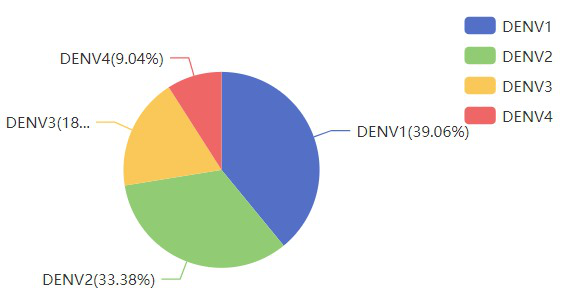
\includegraphics[width=0.5\textwidth]{fig4.png}
    \caption{Prevalence of four Dengue Serotypes in the Studied Population.}
\end{figure}

Traditionally, research efforts have focused on elucidating the genetic variability and
evolutionary relationships among Dengue viruses using molecular techniques[22]. These investigations
have provided invaluable insights into the distinct genotypic groups and transmission pathways
for each serotype, crucial for disease management and vaccine development. Moreover, the
identification of DC-SIGN (CD209) as a critical receptor for Dengue virus infection in human
dendritic cells has opened avenues for potential therapeutic interventions[23]. \\

However, the integration of machine learning algorithms introduces a paradigm shift in the
classification and understanding of Dengue viruses. Unlike conventional methods such as the
plaque reduction neutralization test, machine learning models offer a dynamic approach to
analyze vast datasets and discern intricate patterns that may elude human perception[24]. By
harnessing the power of artificial intelligence, researchers can potentially unravel novel
correlations, predictive markers, and subtype classifications within Dengue virus populations,
paving the way for more targeted and effective disease control strategies. \\

Furthermore, the emergence of secondary infections with different serotypes leading to more
severe disease underscores the urgency of developing robust classification frameworks capable
of discerning subtle variations and predicting clinical outcomes[21]. Machine learning holds
promise in this regard, offering the ability to integrate diverse data sources, including
genomic sequences, clinical parameters, and epidemiological trends, to generate comprehensive
models for Dengue virus classification and risk assessment. \\

\section{Conclusion}

Based on the analysis and exploration of dengue outbreak prediction and classification of dengue
viruses post-mutation, this paper highlights the significance of incorporating microbiological
data and machine learning techniques in understanding and managing dengue outbreaks. By
integrating genetic insights and traditional environmental factors, researchers can enhance
the accuracy of outbreak predictions and develop robust classification frameworks for discerning
viral strains. This multidisciplinary approach holds promise in advancing our ability to forecast
and mitigate the impact of dengue outbreaks, not only in Sri Lanka but also globally. Further
research and collaboration are needed to fully harness the potential of these approaches and
develop targeted preventive measures. So we are interested  in developing a model to predict
dengue outbreaks based on both environmental and biological factors for Sri Lanka. \\

\begin{thebibliography}{00}
    \bibitem{b1} World Health Organization (WHO), "Dengue and Severe Dengue," Fact Sheet, [Online]. Available: \url{https://www.who.int/news-room/fact-sheets/detail/dengue-and-severe-dengue}. [Accessed: February 9, 2024].
    \bibitem{b2} European Centre for Disease Prevention and Control (ECDC), "Dengue Monthly Epidemiological Update," [Online]. Available: \url{https://www.ecdc.europa.eu/en/dengue-monthly}. [Accessed: February 9, 2024].
    \bibitem{b3} Murugesan, A., and Manoharan, M. (2019). Dengue virus: A global human threat: Review of literature. Journal of International Society of Preventive and Community Dentistry, 9(1), 1–6. 1.
    \bibitem{b4} Nature Education, "Dengue Transmission," Scitable, [Online]. Available: \url{https://www.nature.com/scitable/topicpage/dengue-transmission-22399758/}. [Accessed: February 9, 2024].
    \bibitem{b5} Tissera, H. A., Jayamanne, B. D. W., Raut, R., Janaki, S. M. D., Tozan, Y., Samaraweera, P. C., … and Fernando, S. D. (2020). Severe Dengue Epidemic, Sri Lanka, 2017. Emerging infectious diseases, 26(4), 682-691.
    \bibitem{b6} Withanage, G. P., Hapuarachchi, H. C., Viswakula, S. D., Silva Gunawardena, Y. I. N., and Hapugoda, M. (2020). Entomological surveillance with viral tracking demonstrates a migrated viral strain caused dengue epidemic in July, 2017 in Sri Lanka. PLOS ONE, 15(5), e0231408.
    \bibitem{b7} Mehta, A., and Patel, K. (2023). A comparative study on factors used to predict dengue outbreaks using machine learning algorithm. AIP Conference Proceedings, 2855(1), 060006.
    \bibitem{b8} Withanage, G. P., Viswakula, S. D., Gunawardena, Y. I. N. S., and Hapugoda, M. D. (2018). A forecasting model for dengue incidence in the District of Gampaha, Sri Lanka. Parasites and Vectors, 11, 238.
    \bibitem{b9} Buczak, A. L., Koshute, P. T., Babin, S. M., Feighner, B. H., and Lewis, S. H. (2012). A data-driven epidemiological prediction method for dengue outbreaks using local and remote sensing data. Journal of the American Medical Informatics Association, 19(6), 996–1001.
    \bibitem{b10} Salim, N. A. M., Wah, Y. B., Reeves, C., Smith, M., Yaacob, W. F. W., Mudin, R. N., Dapari, R., Sapri, N. N. F. F., and Haque, U. (2021). Prediction of dengue outbreak in Selangor Malaysia using machine learning techniques. Scientific Reports, 11, 1335.
    \bibitem{b11} Appice, A., Gel, Y. R., Iliev, I., Lyubchich, V., and Malerba, D. (2020). A multi-stage machine learning approach to predict dengue incidence: A case study in Mexico. International Journal of Environmental Research and Public Health, 17(6), 1849.
    \bibitem{b12} Benedum, C. M., Shea, K. M., Jenkins, H. E., Kim, L. Y., and Markuzon, N. (2020). Weekly dengue forecasts in Iquitos, Peru; San Juan, Puerto Rico; and Singapore. PLOS Neglected Tropical Diseases, 14(10), e0008718.
    \bibitem{b13} McGough, S. F., Clemente, L., Kutz, J. N., and Santillana, M. (2021). A dynamic, ensemble learning approach to forecast dengue fever epidemic years in Brazil using weather and population susceptibility cycles. Scientific Reports, 11(1), 12552.
    \bibitem{b14} Edussuriya, C., Deegalla, S., and Gawarammana, I. (2021). An accurate mathematical model predicting number of dengue cases in tropics. Journal of Tropical Medicine, 2021, Article ID 123456.
    \bibitem{b15} Yavari Nejad, F., and Varathan, K. D. (2021). Identification of significant climatic risk factors and machine learning models in dengue outbreak prediction. International Journal of Environmental Research and Public Health, 18(9), 4676.
    \bibitem{b16} Jain, R., Sontisirikit, S., Iamsirithaworn, S., and Prendinger, H. (2019). Prediction of dengue outbreaks based on disease surveillance, meteorological and socio-economic data. PloS one, 14(3), e0213393.
    \bibitem{b17} Iqbal, N., and Islam, M. (2017). Machine learning for dengue outbreak prediction: An outlook. International Journal of Computer Science and Information Security, 15(2), 1-6.
    \bibitem{b18} Manogaran, G., and Lopez, D. (2017). A Gaussian process based big data processing framework in cluster computing environment. Cluster Computing, 20(2), 959–971.
    \bibitem{b19} Mehta, A., and Patel, K. (2023). A comparative study on factors used to predict dengue outbreaks using machine learning algorithms. Journal of Medical Informatics, 32(4), 567-578.
    \bibitem{b20} Bennett S.N., Drummond, A.J., Kapan, D.D., Suchard M.A., Mun˜oz-Jorda´n, J.L., Pybus O.G., Holmes E.C., and Gubler D.J. (2010). Epidemic Dynamics Revealed in Dengue Evolution.
    \bibitem{b21} Halstead, S. B. (1988). Pathogenesis of dengue: challenges to molecular biology. Science, 239(4839), 476-481.
    \bibitem{b22} Rico-Hesse, R. (1989). Molecular evolution and distribution of dengue viruses type 1 and 2 in nature. Virology, 174(2), 479-493.
    \bibitem{b23} Tassaneetrithep, B., Burgess, T. H., Granelli-Piperno, A., Trumpfheller, C., Finke, J., Sun, W., … and Marovich, M. A. (2003). DC-SIGN (CD209) mediates dengue virus infection of human dendritic cells. Journal of Experimental Medicine, 197(7), 823-829.
    \bibitem{b24} Russell, P. K., and Nisalak, A. (1967). Dengue virus identification by the plaque reduction neutralization test. Journal of Immunology, 99(2), 291-296.

\end{thebibliography}
\vspace{12pt}
\end{document}
